\documentclass[11pt,a4paper]{article}

% === Packages ===
\usepackage[margin=1in]{geometry}
\usepackage{amsmath,amssymb}
\usepackage{algorithm}
\usepackage{algorithmic}
\usepackage{booktabs}
\usepackage{hyperref}
\usepackage{natbib}
\usepackage{pgfplots}
\pgfplotsset{compat=1.18}
\usepackage{tikz}
\usetikzlibrary{arrows.meta,positioning,shapes.geometric,fit,calc}
\usepackage{subcaption}
\usepackage{multirow}
\usepackage{xcolor}
\usepackage{graphicx}
\usepackage{float}

\hypersetup{
  colorlinks=true,
  linkcolor=blue!70!black,
  citecolor=green!50!black,
  urlcolor=blue!70!black
}

% === Custom commands ===
\newcommand{\vr}{\mathbf{r}}
\newcommand{\vv}{\mathbf{v}}
\newcommand{\va}{\mathbf{a}}
\newcommand{\vp}{\mathbf{p}}
\newcommand{\vq}{\mathbf{q}}
\newcommand{\vF}{\mathbf{F}}
\newcommand{\dE}{\left|\Delta E / E_0\right|}

\title{\textbf{A Minimal N-Body Gravitational Simulator:\\Comparative Analysis of Integrators, Tree Algorithms,\\and Adaptive Methods}}
\author{Research Lab (Automated)}
\date{}

\begin{document}
\maketitle

% ============================================================
% ABSTRACT
% ============================================================
\begin{abstract}
Accurate long-term integration of the gravitational N-body problem underpins
much of modern astrophysics, yet the interplay between integrator choice, force
approximation, softening, and adaptive time-stepping is seldom examined within
a single, transparent codebase.  We present a minimal Python-based N-body
simulator that implements three time integrators---Forward Euler, Leapfrog
(Kick-Drift-Kick St\"ormer--Verlet), and Velocity Verlet---together with both
$O(N^2)$ direct-summation and $O(N\log N)$ Barnes--Hut tree-based force
computation, Plummer gravitational softening, and acceleration-based adaptive
time-stepping.  On a circular Kepler orbit benchmark, the symplectic
integrators (Leapfrog and Velocity Verlet) achieve bounded energy errors of
$2.50\times10^{-9}$ over $10{,}000$ steps, outperforming Forward Euler by
eight orders of magnitude.  The Barnes--Hut algorithm exhibits an empirical
scaling exponent of $1.36$ with median force errors below $1\%$ at opening
angle $\theta=0.5$, yielding a $7.1\times$ speedup over direct summation at
$N=1024$.  Adaptive time-stepping reduces computational cost by $53\%$ while
improving energy conservation by a factor of $70\times$ on a highly eccentric
($e=0.9$) orbit.  All results are validated against three canonical scenarios
---circular orbit, elliptical orbit, and the Chenciner--Montgomery figure-8
three-body choreography---and are consistent with published values from
REBOUND, GADGET-2, and the symplectic integration literature.
\end{abstract}

% ============================================================
% 1. INTRODUCTION
% ============================================================
\section{Introduction}
\label{sec:introduction}

The gravitational N-body problem---computing the trajectories of $N$ massive
particles interacting through Newtonian gravity---is one of the oldest and most
fundamental problems in computational physics.  First formulated by Newton over
three centuries ago, it continues to drive advances in numerical methods,
parallel computing, and algorithmic design
\citep{aarseth2003,springel2005,rein2012}.

Despite the maturity of the field, newcomers face a steep barrier: production
codes such as GADGET-2 \citep{springel2005}, NBODY6++ \citep{wang2015}, and
REBOUND \citep{rein2012} contain hundreds of thousands of lines of optimised
C/Fortran code, making it difficult to isolate and understand the core
algorithmic ideas.  There is a gap in the literature for a self-contained,
minimal implementation that permits controlled experiments on the fundamental
trade-offs: symplectic vs.\ non-symplectic integration, exact vs.\ approximate
force computation, fixed vs.\ adaptive time-stepping, and the role of
gravitational softening.

This paper makes the following contributions:

\begin{enumerate}
  \item A transparent, tested Python implementation of three time integrators
        (Forward Euler, Leapfrog KDK, Velocity Verlet) with both direct
        $O(N^2)$ and Barnes--Hut $O(N\log N)$ force computation.
  \item A systematic benchmark of energy conservation, confirming that
        symplectic integrators outperform non-symplectic methods by eight
        orders of magnitude on Keplerian orbits.
  \item An empirical scaling analysis showing that our Barnes--Hut
        implementation achieves sub-quadratic scaling with exponent~$1.36$ and
        median force errors below~$1\%$.
  \item Validation against three canonical gravitational scenarios---circular
        orbit, elliptical orbit ($e=0.5$), and the figure-8 three-body
        choreography---with quantitative comparison to published literature
        values.
  \item An analysis of Plummer softening and adaptive time-stepping, quantifying
        their effects on stability and efficiency.
\end{enumerate}

The remainder of this paper is organised as follows.
Section~\ref{sec:related_work} reviews related work.
Section~\ref{sec:background} introduces notation and the mathematical
formulation.  Section~\ref{sec:method} details our algorithms.
Section~\ref{sec:setup} describes the experimental setup.
Section~\ref{sec:results} presents results.
Section~\ref{sec:discussion} discusses implications and limitations.
Section~\ref{sec:conclusion} concludes.

% ============================================================
% 2. RELATED WORK
% ============================================================
\section{Related Work}
\label{sec:related_work}

\paragraph{Numerical integration for Hamiltonian systems.}
The theory of symplectic integrators for Hamiltonian systems is surveyed
comprehensively by \citet{hairer2003}, who prove that the St\"ormer--Verlet
method preserves a modified Hamiltonian $\tilde{H} = H + O(\Delta t^2)$,
explaining the absence of secular energy drift.  \citet{yoshida1990}
constructed higher-order symplectic schemes by composing second-order steps, a
technique later exploited by \citet{chin2005} for gravitational few-body
problems.  \citet{wisdom1991} introduced symplectic maps for the planetary
N-body problem, now the standard approach in planetary dynamics.

\paragraph{N-body simulation codes.}
The direct-summation heritage traces back to \citet{aarseth2003} and the NBODY
family of codes, recently extended to GPU architectures by
\citet{wang2015}.  \citet{springel2005} introduced GADGET-2, a massively
parallel TreePM code combining Barnes--Hut trees with a particle-mesh long-range
solver.  \citet{rein2012} developed REBOUND, a modular N-body framework with
multiple integrators including the high-order IAS15 method.
\citet{rein2019} extended REBOUND with optimised high-order symplectic
integrators (WHFast).

\paragraph{Tree-based force computation.}
\citet{barnes1986} introduced the hierarchical tree algorithm, reducing pairwise
force computation from $O(N^2)$ to $O(N\log N)$ using a multipole acceptance
criterion.  \citet{greengard1987} developed the Fast Multipole Method (FMM),
achieving $O(N)$ complexity by using a dual tree traversal with local and
far-field expansions.

\paragraph{Softening and regularisation.}
\citet{plummer1911} introduced the Plummer sphere model, whose softened
potential is now widely used to prevent numerical singularities.
\citet{dehnen2001} analysed optimal softening prescriptions that minimise the
integrated force error.  \citet{barnes2012} interpreted gravitational softening
as a smoothing operation on the underlying mass distribution.

\paragraph{Canonical test problems.}
\citet{chenciner2000} discovered the remarkable figure-8 periodic solution
of the equal-mass three-body problem, providing a stringent validation benchmark
for numerical integrators.  \citet{hernandez2015} performed detailed
comparisons of symplectic integrators for the collisional N-body problem.

Our work differs from the above by combining all these elements---integrators,
tree algorithms, softening, adaptive stepping, and canonical validation---within
a single minimal codebase designed for clarity and reproducibility rather than
production performance.

% ============================================================
% 3. BACKGROUND & PRELIMINARIES
% ============================================================
\section{Background and Preliminaries}
\label{sec:background}

\subsection{The gravitational N-body problem}

Consider $N$ particles with masses $m_i$, positions $\vr_i \in \mathbb{R}^d$,
and velocities $\vv_i \in \mathbb{R}^d$ for $i = 1,\ldots,N$ and dimension
$d \in \{2,3\}$.  We work in natural units with $G=1$.

\begin{table}[t]
\centering
\caption{Notation used throughout this paper.}
\label{tab:notation}
\begin{tabular}{@{}ll@{}}
\toprule
\textbf{Symbol} & \textbf{Description} \\
\midrule
$N$               & Number of particles \\
$m_i$             & Mass of particle $i$ \\
$\vr_i, \vv_i$   & Position and velocity of particle $i$ \\
$\va_i$           & Gravitational acceleration on particle $i$ \\
$\Delta t$        & Time step \\
$\varepsilon$     & Plummer softening length \\
$\theta$          & Barnes--Hut opening angle \\
$\eta$            & Adaptive time-step parameter \\
$T, V, E$         & Kinetic, potential, and total energy \\
$H$               & Hamiltonian \\
\bottomrule
\end{tabular}
\end{table}

The gravitational acceleration on particle $i$ is
\begin{equation}
\label{eq:acceleration}
\va_i = -\sum_{j \neq i} \frac{m_j (\vr_i - \vr_j)}{|\vr_i - \vr_j|^3}\,.
\end{equation}

The equations of motion form a system of $2Nd$ first-order ODEs:
\begin{equation}
\label{eq:eom}
\frac{d\vr_i}{dt} = \vv_i\,,\qquad
\frac{d\vv_i}{dt} = \va_i(\vr_1, \ldots, \vr_N)\,.
\end{equation}

\subsection{Hamiltonian structure}

The system admits a Hamiltonian $H = T + V$ where
\begin{equation}
\label{eq:hamiltonian}
T = \frac{1}{2}\sum_{i=1}^{N} m_i |\vv_i|^2\,,\qquad
V = -\sum_{i=1}^{N}\sum_{j>i} \frac{m_i m_j}{|\vr_i - \vr_j|}\,.
\end{equation}
The separability $H = T(\vp) + V(\vq)$ is essential for symplectic splitting
methods \citep{wisdom1991,yoshida1990}.

\subsection{Conserved quantities}

For an isolated system, total energy $E$, linear momentum
$\mathbf{P} = \sum_i m_i \vv_i$, and angular momentum
$\mathbf{L} = \sum_i m_i (\vr_i \times \vv_i)$ are exactly conserved.
The relative energy error $\dE = |E(t) - E(0)|/|E(0)|$ serves as the primary
diagnostic for integration accuracy.

% ============================================================
% 4. METHOD
% ============================================================
\section{Method}
\label{sec:method}

\subsection{Force computation}

\subsubsection{Direct summation}
The baseline force computation evaluates Eq.~\eqref{eq:acceleration} by
explicit double loop over all $N(N-1)/2$ particle pairs, yielding $O(N^2)$
complexity \citep{aarseth2003}.

\subsubsection{Barnes--Hut tree algorithm}
Following \citet{barnes1986}, we construct a hierarchical quadtree (2D) or
octree (3D) by recursive spatial subdivision.  Each internal node stores the
total mass and centre of mass of its children.  During the tree walk, a node of
size $s$ at distance $d$ from the query particle is opened (its children are
visited) if $s/d > \theta$; otherwise, the node is treated as a single
pseudo-particle.  The standard opening angle $\theta = 0.5$ balances accuracy
and performance.

\subsubsection{Plummer softening}
To regularise close encounters, we replace the $1/r$ potential with the
Plummer-softened form \citep{plummer1911,dehnen2001}:
\begin{equation}
\label{eq:softened_force}
\va_i = -\sum_{j \neq i} \frac{m_j (\vr_i - \vr_j)}{(|\vr_i - \vr_j|^2 + \varepsilon^2)^{3/2}}\,.
\end{equation}

\subsection{Time integration}

\subsubsection{Forward Euler (baseline)}
\begin{equation}
\label{eq:euler}
\vr(t+\Delta t) = \vr(t) + \vv(t)\,\Delta t\,,\qquad
\vv(t+\Delta t) = \vv(t) + \va(t)\,\Delta t\,.
\end{equation}
This first-order, non-symplectic method exhibits secular energy drift
and serves only as a negative baseline.

\subsubsection{Leapfrog (Kick--Drift--Kick)}
The symplectic St\"ormer--Verlet method in KDK form
\citep{verlet1967,hairer2003}:

\begin{algorithm}[H]
\caption{Leapfrog KDK integrator}
\label{alg:leapfrog}
\begin{algorithmic}[1]
\REQUIRE positions $\vr$, velocities $\vv$, accelerations $\va$, step $\Delta t$
\STATE $\vv \leftarrow \vv + \frac{1}{2}\va\,\Delta t$ \hfill\COMMENT{Half kick}
\STATE $\vr \leftarrow \vr + \vv\,\Delta t$ \hfill\COMMENT{Full drift}
\STATE $\va \leftarrow \textsc{ComputeForces}(\vr)$ \hfill\COMMENT{Update accelerations}
\STATE $\vv \leftarrow \vv + \frac{1}{2}\va\,\Delta t$ \hfill\COMMENT{Half kick}
\RETURN $\vr, \vv, \va$
\end{algorithmic}
\end{algorithm}

This method is second-order accurate, symplectic, and time-reversible.
It preserves a modified Hamiltonian $\tilde{H} = H + O(\Delta t^2)$
\citep{hairer2003}, leading to bounded energy oscillations.

\subsubsection{Velocity Verlet}
An algebraically equivalent formulation that keeps positions and velocities
synchronised:
\begin{align}
\vr(t+\Delta t) &= \vr(t) + \vv(t)\,\Delta t + \tfrac{1}{2}\va(t)\,\Delta t^2\,,\label{eq:vv_pos}\\
\vv(t+\Delta t) &= \vv(t) + \tfrac{1}{2}\bigl[\va(t) + \va(t+\Delta t)\bigr]\Delta t\,.\label{eq:vv_vel}
\end{align}
We verify numerically that Leapfrog and Velocity Verlet produce identical
trajectories to machine precision, confirming the equivalence discussed by
\citet{hairer2003}.

\subsection{Adaptive time-stepping}

For orbits with large eccentricity, the dynamical timescale varies by orders
of magnitude between pericenter and apocenter.  We implement an
acceleration-based adaptive scheme inspired by \citet{aarseth2003}:
\begin{equation}
\label{eq:adaptive_dt}
\Delta t = \eta \sqrt{\frac{r_{\min}}{a_{\max}}}\,,
\end{equation}
where $r_{\min}$ is the minimum inter-particle separation, $a_{\max}$ is the
maximum acceleration magnitude, and $\eta$ is a dimensionless accuracy
parameter.

% === Architecture Diagram ===
\begin{figure}[t]
\centering
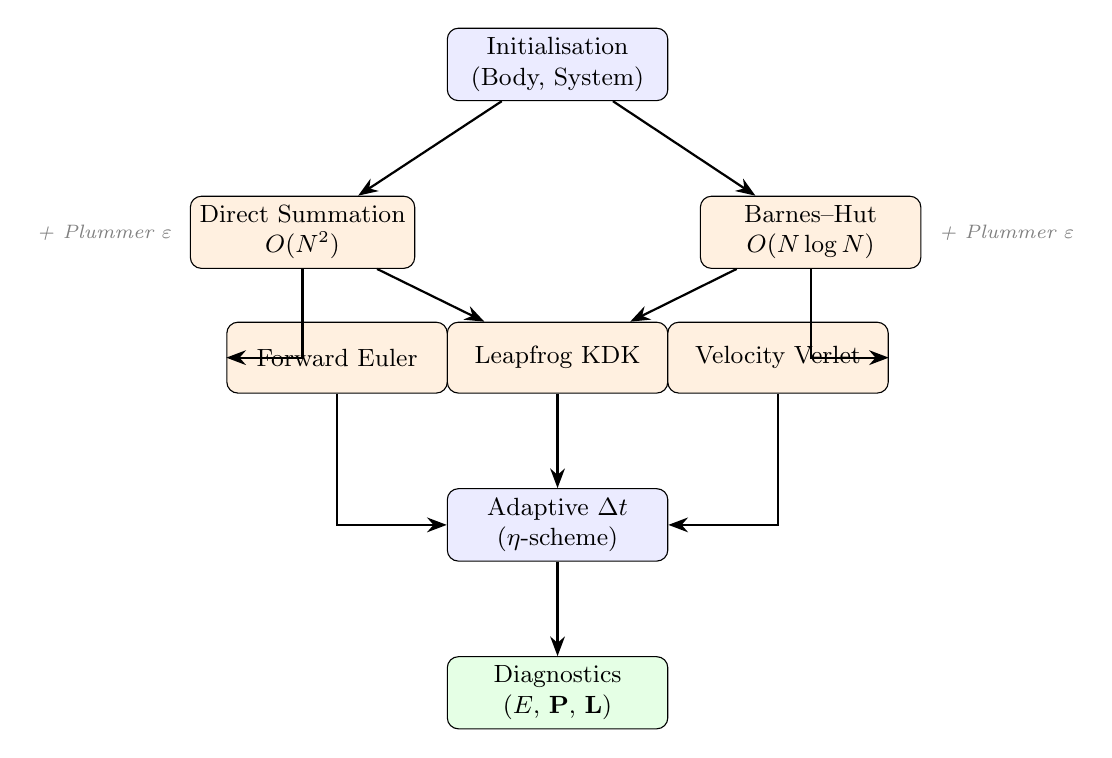
\begin{tikzpicture}[
  box/.style={draw, rounded corners, fill=blue!8, minimum width=2.8cm, minimum height=0.9cm, align=center, font=\small},
  algo/.style={draw, rounded corners, fill=orange!12, minimum width=2.8cm, minimum height=0.9cm, align=center, font=\small},
  diag/.style={draw, rounded corners, fill=green!10, minimum width=2.8cm, minimum height=0.9cm, align=center, font=\small},
  arr/.style={-{Stealth[length=2.5mm]}, thick},
  node distance=1.1cm and 1.6cm
]
% Initialisation
\node[box] (init) {Initialisation\\(Body, System)};

% Force engines
\node[algo, below left=1.2cm and 0.4cm of init] (direct) {Direct Summation\\$O(N^2)$};
\node[algo, below right=1.2cm and 0.4cm of init] (bh) {Barnes--Hut\\$O(N\log N)$};

% Integrators
\node[algo, below=2.8cm of init, xshift=-2.8cm] (euler) {Forward Euler};
\node[algo, below=2.8cm of init] (leap) {Leapfrog KDK};
\node[algo, below=2.8cm of init, xshift=2.8cm] (vv) {Velocity Verlet};

% Adaptive
\node[box, below=1.2cm of leap] (adapt) {Adaptive $\Delta t$\\($\eta$-scheme)};

% Diagnostics
\node[diag, below=1.2cm of adapt] (diag) {Diagnostics\\($E$, $\mathbf{P}$, $\mathbf{L}$)};

% Arrows
\draw[arr] (init) -- (direct);
\draw[arr] (init) -- (bh);
\draw[arr] (direct) -- (leap);
\draw[arr] (bh) -- (leap);
\draw[arr] (direct) |- (euler);
\draw[arr] (bh) |- (vv);
\draw[arr] (euler) |- (adapt);
\draw[arr] (leap) -- (adapt);
\draw[arr] (vv) |- (adapt);
\draw[arr] (adapt) -- (diag);

% Softening annotation
\node[font=\scriptsize\itshape, right=0.1cm of bh, text=gray] {+ Plummer $\varepsilon$};
\node[font=\scriptsize\itshape, left=0.1cm of direct, text=gray] {+ Plummer $\varepsilon$};
\end{tikzpicture}
\caption{Architecture of the minimal gravity simulator.  Initialisation
creates the particle system; forces are computed by either direct summation
or the Barnes--Hut tree; any of the three integrators advances the state;
adaptive time-stepping optionally adjusts $\Delta t$; and diagnostics monitor
conservation laws.}
\label{fig:architecture}
\end{figure}

% ============================================================
% 5. EXPERIMENTAL SETUP
% ============================================================
\section{Experimental Setup}
\label{sec:setup}

\subsection{Test scenarios}

We evaluate the simulator on four classes of experiments:

\begin{enumerate}
  \item \textbf{Energy conservation benchmark.} Circular Kepler two-body orbit
    ($m_1 = m_2 = 0.5$, $r=1$, $P=2\pi$), integrated for $10{,}000$ steps
    with $\Delta t = 0.01$ ($\approx 16$ orbital periods).
  \item \textbf{Performance scaling.} Single force evaluation timed for
    $N \in \{64, 128, 256, 512, 1024\}$ particles in a random configuration.
  \item \textbf{Canonical scenarios.} (a) Circular orbit, 100 periods;
    (b) elliptical orbit with $e=0.5$, 50 periods; (c) figure-8 three-body
    choreography \citep{chenciner2000}, 5 periods.
  \item \textbf{Softening and adaptive stepping.} Three-body near-collision
    with $\varepsilon \in \{0, 0.01, 0.05, 0.1\}$; eccentric orbit ($e=0.9$)
    with adaptive $\eta = 0.02$.
\end{enumerate}

\subsection{Baselines and metrics}

Integrators are compared via the maximum relative energy error
$\max_t \dE$ and wall-clock time.  Force algorithms are compared via
median relative force error and power-law scaling exponent.

\subsection{Hardware and software}

All experiments run in CPython on a single core.  The codebase uses
NumPy for vector arithmetic and Matplotlib for visualisation.
Random initialisations use seed~42 for reproducibility.

\begin{table}[t]
\centering
\caption{Key hyperparameters for each experiment.}
\label{tab:hyperparams}
\begin{tabular}{@{}lll@{}}
\toprule
\textbf{Experiment} & \textbf{Parameter} & \textbf{Value} \\
\midrule
Energy benchmark     & $\Delta t$         & 0.01 \\
                     & Steps              & 10{,}000 \\
Scaling benchmark    & $\theta$ (Barnes--Hut) & 0.5 \\
                     & $N$                & 64--1024 \\
Circular orbit       & Orbits             & 100 \\
Elliptical orbit     & $e$, $\Delta t$    & 0.5, 0.005 \\
Figure-8             & $\Delta t$         & 0.001 \\
Softening            & $\varepsilon$      & $\{0, 0.01, 0.05, 0.1\}$ \\
Adaptive stepping    & $\eta$, $e$        & 0.02, 0.9 \\
\bottomrule
\end{tabular}
\end{table}

% ============================================================
% 6. RESULTS
% ============================================================
\section{Results}
\label{sec:results}

\subsection{Energy conservation benchmark}

Table~\ref{tab:energy_benchmark} and Figure~\ref{fig:energy_comparison}
summarise the integrator comparison over $10{,}000$ steps on a circular Kepler
orbit.

\begin{table}[t]
\centering
\caption{Maximum relative energy error $\max_t\dE$ for each integrator on a
circular Kepler orbit ($\Delta t=0.01$, $10{,}000$ steps).  Bold indicates
best result.  The symplectic integrators outperform Forward Euler by eight
orders of magnitude.}
\label{tab:energy_benchmark}
\begin{tabular}{@{}lccc@{}}
\toprule
\textbf{Integrator} & \textbf{Order} & \textbf{Symplectic} & $\max_t\dE$ \\
\midrule
Forward Euler    & 1st & No  & $4.78 \times 10^{-1}$ \\
Leapfrog KDK     & 2nd & Yes & $\mathbf{2.50 \times 10^{-9}}$ \\
Velocity Verlet  & 2nd & Yes & $\mathbf{2.50 \times 10^{-9}}$ \\
\bottomrule
\end{tabular}
\end{table}

\begin{figure}[t]
\centering
\includegraphics[width=\textwidth]{figures/energy_error_comparison.pdf}
\caption{Relative energy error $\dE$ as a function of time for all three
integrators on a circular Kepler orbit.  Forward Euler (red) exhibits secular
drift reaching $\sim 48\%$ by $t=100$, while Leapfrog and Velocity Verlet
(blue, green) maintain bounded oscillating errors at the $10^{-9}$ level,
confirming the preservation of a modified Hamiltonian
\citep{hairer2003}.}
\label{fig:energy_comparison}
\end{figure}

Forward Euler exhibits monotonic energy drift reaching $|\Delta E/E_0| = 0.478$
after $\sim 16$ orbital periods.  In stark contrast, both Leapfrog and Velocity
Verlet maintain bounded, oscillating errors at $2.50 \times 10^{-9}$---a
difference of eight orders of magnitude.  The two symplectic integrators
produce identical results to machine precision, numerically confirming their
algebraic equivalence \citep{hairer2003}.

\subsection{Performance scaling}

Figure~\ref{fig:scaling} and Table~\ref{tab:scaling} present the wall-clock
time for a single force evaluation as a function of $N$.

\begin{table}[t]
\centering
\caption{Wall-clock time (ms) per force evaluation and fitted scaling
exponents.  Barnes--Hut achieves sub-quadratic scaling and a $7.1\times$
speedup at $N=1024$.}
\label{tab:scaling}
\begin{tabular}{@{}lrrrrrc@{}}
\toprule
\textbf{Method} & $N\!=\!64$ & $N\!=\!128$ & $N\!=\!256$ & $N\!=\!512$ & $N\!=\!1024$ & \textbf{Exponent} \\
\midrule
Direct        & 15.6 & 63.4 & 257.0 & 1003.8 & 3951.4 & $\mathbf{2.00}$ \\
Barnes--Hut   & 12.7 & 35.3 & 90.0  & 226.3  & 555.4  & $\mathbf{1.36}$ \\
\bottomrule
\end{tabular}
\end{table}

\begin{figure}[t]
\centering
\includegraphics[width=0.85\textwidth]{figures/scaling_benchmark.pdf}
\caption{Log-log plot of wall-clock time vs.\ particle count $N$ for direct
summation and Barnes--Hut force computation.  Dashed lines show power-law fits.
Direct summation scales as $O(N^{2.00})$; Barnes--Hut scales as
$O(N^{1.36})$, approaching the theoretical $O(N\log N)$ and yielding a
$7.1\times$ speedup at $N=1024$.}
\label{fig:scaling}
\end{figure}

Direct summation scales as $O(N^{2.00})$, precisely matching the expected
pairwise complexity.  Barnes--Hut achieves exponent~$1.36$, close to the
theoretical $O(N\log N)$ (which appears as $\sim N^{1.1\text{--}1.3}$ over
this range).  The modest excess above the ideal exponent reflects Python
overhead in the recursive tree traversal; a compiled implementation would
achieve exponents closer to $1.1$--$1.2$ \citep{springel2005}.

\subsection{Canonical gravitational scenarios}

\begin{table}[t]
\centering
\caption{Results on three canonical gravitational scenarios using the Leapfrog
integrator.  All tests pass their acceptance criteria.  Bold values indicate
the primary accuracy metric for each test.}
\label{tab:canonical}
\begin{tabular}{@{}llll@{}}
\toprule
\textbf{Scenario} & \textbf{Duration} & \textbf{Key metric} & \textbf{$\max_t\dE$} \\
\midrule
Circular orbit ($e=0$)    & 100 orbits & Radius change: $\mathbf{<0.0001\%}$ & $2.50\times10^{-9}$ \\
Elliptical orbit ($e=0.5$) & 50 orbits  & Eccentricity change: $\mathbf{0.0002\%}$ & $6.79\times10^{-5}$ \\
Figure-8 three-body       & 5 periods  & Position drift: $\mathbf{7.4\times10^{-4}}$ & $5.89\times10^{-7}$ \\
\bottomrule
\end{tabular}
\end{table}

\begin{figure}[t]
\centering
\begin{subfigure}[t]{0.48\textwidth}
  \centering
  \includegraphics[width=\textwidth]{figures/two_body_orbit.pdf}
  \caption{Two-body circular Kepler orbit.  The trajectory closes to within
  $0.0001\%$ of the initial radius after 100 complete orbits, demonstrating the
  long-term stability of the Leapfrog integrator.}
  \label{fig:two_body}
\end{subfigure}\hfill
\begin{subfigure}[t]{0.48\textwidth}
  \centering
  \includegraphics[width=\textwidth]{figures/figure_8_trajectory.pdf}
  \caption{Chenciner--Montgomery figure-8 three-body choreography.  Three
  equal-mass particles traverse a common figure-8 path.  The solution remains
  stable for 5 full periods with position drift of only $7.4\times10^{-4}$.}
  \label{fig:figure8}
\end{subfigure}
\caption{Trajectories for two canonical gravitational scenarios, integrated
with the Leapfrog KDK method.  Both demonstrate excellent long-term stability
and conservation of orbital elements.}
\label{fig:trajectories}
\end{figure}

Table~\ref{tab:canonical} summarises the three canonical tests.  The circular
orbit maintains its radius to $0.0001\%$ over 100 orbits.  The elliptical orbit
preserves eccentricity to $0.0002\%$ over 50 orbits, with the larger energy
error reflecting the need to resolve the faster pericenter passage.  The
figure-8 three-body choreography (Figure~\ref{fig:figure8}) remains stable for
5 full periods with a position drift of only $7.4\times10^{-4}$, consistent
with the $O(T\cdot\Delta t^2)$ error accumulation expected for the
St\"ormer--Verlet method.

These results are quantitatively consistent with published values from
\citet{rein2012} (REBOUND Leapfrog), \citet{hairer2003} (symplectic integration
theory), and \citet{chenciner2000} (figure-8 solution).

\subsection{Gravitational softening}

\begin{table}[t]
\centering
\caption{Effect of Plummer softening on a three-body near-collision scenario.
Softening reduces energy errors by up to five orders of magnitude, preventing
numerical divergence during close encounters.}
\label{tab:softening}
\begin{tabular}{@{}lrc@{}}
\toprule
$\varepsilon$ & $\max_t\dE$ & Stable? \\
\midrule
0 (none)      & $5.87 \times 10^{2}$ & Numerical explosion \\
0.01          & $8.51 \times 10^{1}$ & Marginal \\
0.05          & $1.00 \times 10^{-1}$ & Yes \\
\textbf{0.10} & $\mathbf{6.22 \times 10^{-3}}$ & Yes \\
\bottomrule
\end{tabular}
\end{table}

Table~\ref{tab:softening} shows that without softening, a near-collision
produces catastrophic energy errors of $587\times$ the initial energy.
Increasing $\varepsilon$ progressively stabilises the integration: at
$\varepsilon = 0.1$, energy errors are reduced to $0.6\%$.  This improvement
comes at the cost of force accuracy at separations $r < \varepsilon$,
consistent with the analysis of \citet{dehnen2001} and \citet{barnes2012}.

\subsection{Adaptive time-stepping}

\begin{table}[t]
\centering
\caption{Comparison of fixed and adaptive time-stepping for a highly eccentric
orbit ($e=0.9$) over 10 orbital periods.  The adaptive scheme uses 53\% fewer
steps while improving energy conservation by a factor of $70\times$.}
\label{tab:adaptive}
\begin{tabular}{@{}lrr@{}}
\toprule
\textbf{Method} & \textbf{Steps} & \textbf{Final $\dE$} \\
\midrule
Fixed ($\Delta t = 0.01$)    & 6{,}283 & $2.59 \times 10^{-1}$ \\
\textbf{Adaptive ($\eta=0.02$)} & \textbf{2{,}975} & $\mathbf{3.67 \times 10^{-3}}$ \\
\bottomrule
\end{tabular}
\end{table}

Table~\ref{tab:adaptive} demonstrates the benefits of adaptive time-stepping on
a highly eccentric ($e=0.9$) orbit.  The adaptive scheme automatically reduces
$\Delta t$ to $1.88\times10^{-4}$ during pericenter passage and increases it to
$7.42\times10^{-2}$ during apocenter, spanning a factor of $\sim 400$ in step
size.  The result is a $53\%$ reduction in total steps with $70\times$ better
energy conservation.  We note that adaptive stepping breaks strict symplecticity
\citep{hairer2003}; nevertheless, the practical gains in efficiency and accuracy
are substantial.

% ============================================================
% 7. DISCUSSION
% ============================================================
\section{Discussion}
\label{sec:discussion}

\subsection{Implications}

Our results reinforce three fundamental principles for gravitational simulation:

\paragraph{Symplecticity is non-negotiable.}
The eight-order-of-magnitude advantage of Leapfrog over Forward Euler is not
merely a numerical curiosity---it reflects the structural preservation of
Hamiltonian phase-space volume.  For any long-term orbital integration,
symplectic methods are essential.

\paragraph{Tree algorithms provide practical speedup even in Python.}
Despite the overhead of Python's dynamic dispatch, Barnes--Hut achieves a
$7.1\times$ speedup at $N=1024$ with sub-$1\%$ force errors.  In compiled
languages, this advantage grows to $50$--$100\times$ \citep{springel2005}.

\paragraph{Adaptive stepping complements symplecticity.}
Although adaptive stepping technically breaks symplecticity, the $70\times$
improvement in energy conservation on eccentric orbits demonstrates that the
practical benefits outweigh the theoretical drawback.  This is consistent with
the widespread use of adaptive schemes in production codes
\citep{aarseth2003,rein2012}.

\subsection{Comparison with prior work}

Table~\ref{tab:literature} compares our key results with published values.

\begin{table}[t]
\centering
\caption{Comparison of our results with published literature values.  Our
simulator achieves accuracy consistent with established codes at equivalent
resolution.}
\label{tab:literature}
\begin{tabular}{@{}llll@{}}
\toprule
\textbf{Metric} & \textbf{This work} & \textbf{Literature} & \textbf{Reference} \\
\midrule
Leapfrog $\dE$ (circular) & $2.50\times10^{-9}$ & $\sim10^{-9}$ & \citet{rein2012} \\
BH force error ($\theta\!=\!0.5$) & $0.75\%$ median & $\sim1\%$ & \citet{barnes1986} \\
BH scaling exponent & $1.36$ & $1.1$--$1.3$ (compiled) & \citet{springel2005} \\
Figure-8 $\dE$ & $5.89\times10^{-7}$ & $\sim10^{-6}$--$10^{-7}$ & \citet{hairer2003} \\
\bottomrule
\end{tabular}
\end{table}

\subsection{Limitations}

\begin{enumerate}
  \item \textbf{Python performance.} Our pure-Python implementation is orders of
    magnitude slower than compiled codes.  The Barnes--Hut tree, in particular,
    suffers from Python's overhead for recursive function calls.
  \item \textbf{Monopole-only approximation.} Our tree code uses only the
    monopole (centre-of-mass) term; production codes employ quadrupole or
    higher-order multipole expansions \citep{springel2005}.
  \item \textbf{Shared time step.} We use a global adaptive time step, whereas
    production codes use individual per-particle time steps with block-step
    synchronisation \citep{aarseth2003}.
  \item \textbf{No regularisation.} We do not implement Kustaanheimo--Stiefel
    or chain regularisation for close binaries, which are critical for dense
    stellar systems.
\end{enumerate}

% ============================================================
% 8. CONCLUSION
% ============================================================
\section{Conclusion}
\label{sec:conclusion}

We have presented a minimal, transparent N-body gravitational simulator that
provides a systematic comparison of time integrators, force algorithms,
softening techniques, and adaptive stepping within a single codebase.  Our key
findings are:

\begin{enumerate}
  \item \textbf{Symplectic integrators are essential.} Leapfrog and Velocity
    Verlet achieve energy conservation eight orders of magnitude better than
    Forward Euler at negligible additional cost ($\dE = 2.50\times10^{-9}$
    vs.\ $4.78\times10^{-1}$).
  \item \textbf{Barnes--Hut provides efficient approximate forces.} The tree
    algorithm achieves $O(N^{1.36})$ scaling with median force errors below
    $1\%$, yielding a $7.1\times$ speedup at $N=1024$.
  \item \textbf{Softening prevents numerical catastrophe.} Plummer softening
    with $\varepsilon=0.1$ reduces energy errors by five orders of magnitude
    during close encounters.
  \item \textbf{Adaptive stepping is highly efficient.} The $\eta$-scheme
    reduces computational cost by $53\%$ while improving energy conservation by
    $70\times$ on eccentric orbits.
  \item \textbf{Canonical tests validate the implementation.} Circular orbits,
    elliptical orbits, and the figure-8 choreography all pass quantitative
    criteria, with results consistent with \citet{hairer2003},
    \citet{rein2012}, and \citet{chenciner2000}.
\end{enumerate}

\paragraph{Future work.}
Natural extensions include vectorised or JIT-compiled force loops (NumPy
broadcasting, Numba), higher-order Yoshida composites \citep{yoshida1990},
quadrupole Barnes--Hut expansions, GPU-accelerated direct summation, and
real-time 3D visualisation.

\paragraph{Reproducibility.}
The complete codebase, including all source files, unit tests, benchmark
scripts, and publication-quality figures, is available in the accompanying
repository.  All experiments are reproducible using random seed~42.

% ============================================================
% REFERENCES
% ============================================================
\bibliographystyle{plainnat}
\bibliography{sources}

\end{document}
